\chapter{Dataset configuration management in MADTrack}\label{cap:Milestone1}

This chapter will cover the development of the features described in milestone 1 (codename \emph{D}), which is focused on the development of features related to Dataset
Configuration Management. This module will work in conjuction with the general configuration management module (see \emph{chapter \ref{cap:Milestone3}}) to provide mechianisms
to track and control the changes of the biggest of files. This chapter will introduce the main issues and address the problems to solve to achieve the goals defined for this
milestone.

\section{Introduction}

One of the partial objectives defined for this Final Degree Project involves the development of a module for tracking and versioning datasets. These datasets can be of variable
size, but in many cases bigger than what a free-of-charge configuration management platform can handle. The lack of the existence of a platform that can handle such issue at
at a feasible cost motivates the creation of this dataset tracking module. The main focus of the prototypes of milestone 1 is to provide a mechanism for tracking changes within
datasets, without the need of committing them to the configuration management platform. Another issue to be tackled is that of bringing the correct dataset to the correct environment,
providing at least an interface for this purpose. Firstly, an analysis for the requirements defined for this milestone will be made, separating them by the most suitable
prototypes to be developed, to then proceed to the development details of each of these.

\section{Requirements analysis for milestone 1}

Analysis has the purpose of defining the high-level outline of the application. The definition of this outline requires addressing the question of the most suitable architecture and
application type for the prototypes of this milestone. This analysis will also define the characteristics of a tookit suitable for their development. Furthermore, the
protocol for versioning datasets will also be defined within the analysis phase.

\subsection{Requirements involved}

The requirements involved within this milestone have already been listed within \emph{table \ref{tab:requirementsMilestone1}}. Since this requirements are contained within different prototypes,
it is particularly convenient to define which requirements belong to which prototype. The final requirement division is defined within \

Apart from the final requirement division for each prototype, all prototypes must satisfy the non-functional requirements listed within \emph{table \ref{tab:nonFunctionalRequirements}}.

\subsubsection{Requirements for prototype \emph{D1}}

\begin{table}[H]
    \centering
    \begin{tabular}{ | c | p{9cm} | p{3cm} |}
        \hline
        \textbf{Requirement ID} & \textbf{Requirement Description} & \textbf{priority (MoSCoW)} \\ \hline
        DFR1.2   & The system MUST keep track of the routes where models and datasets are stored    & Must have\\ \hline
    \end{tabular}
\end{table}

\subsubsection{Requirements for prototype \emph{D2}}

\begin{table}[H]
    \centering
    \begin{tabular}{ | c | p{9cm} | p{3cm} |}
        \hline
        \textbf{Requirement ID} & \textbf{Requirement Description} & \textbf{priority (MoSCoW)} \\ \hline
		DFR1     & The system MUST keep ordered track of dataset configurations.                    & Must have\\ \hline
		DFR1.1   & The system MUST detect changes in the size (rows and columns) of datasets.       & Must have\\ \hline
    \end{tabular}
\end{table}

\subsection{Integration with the rest of the system}

Prototypes within milestone 1 only have meaningful interaction with the general configuration management module, mainly because of their dependency from the committing and
checkout methods from milestone 3. 

\begin{figure}[H]
    \centering
    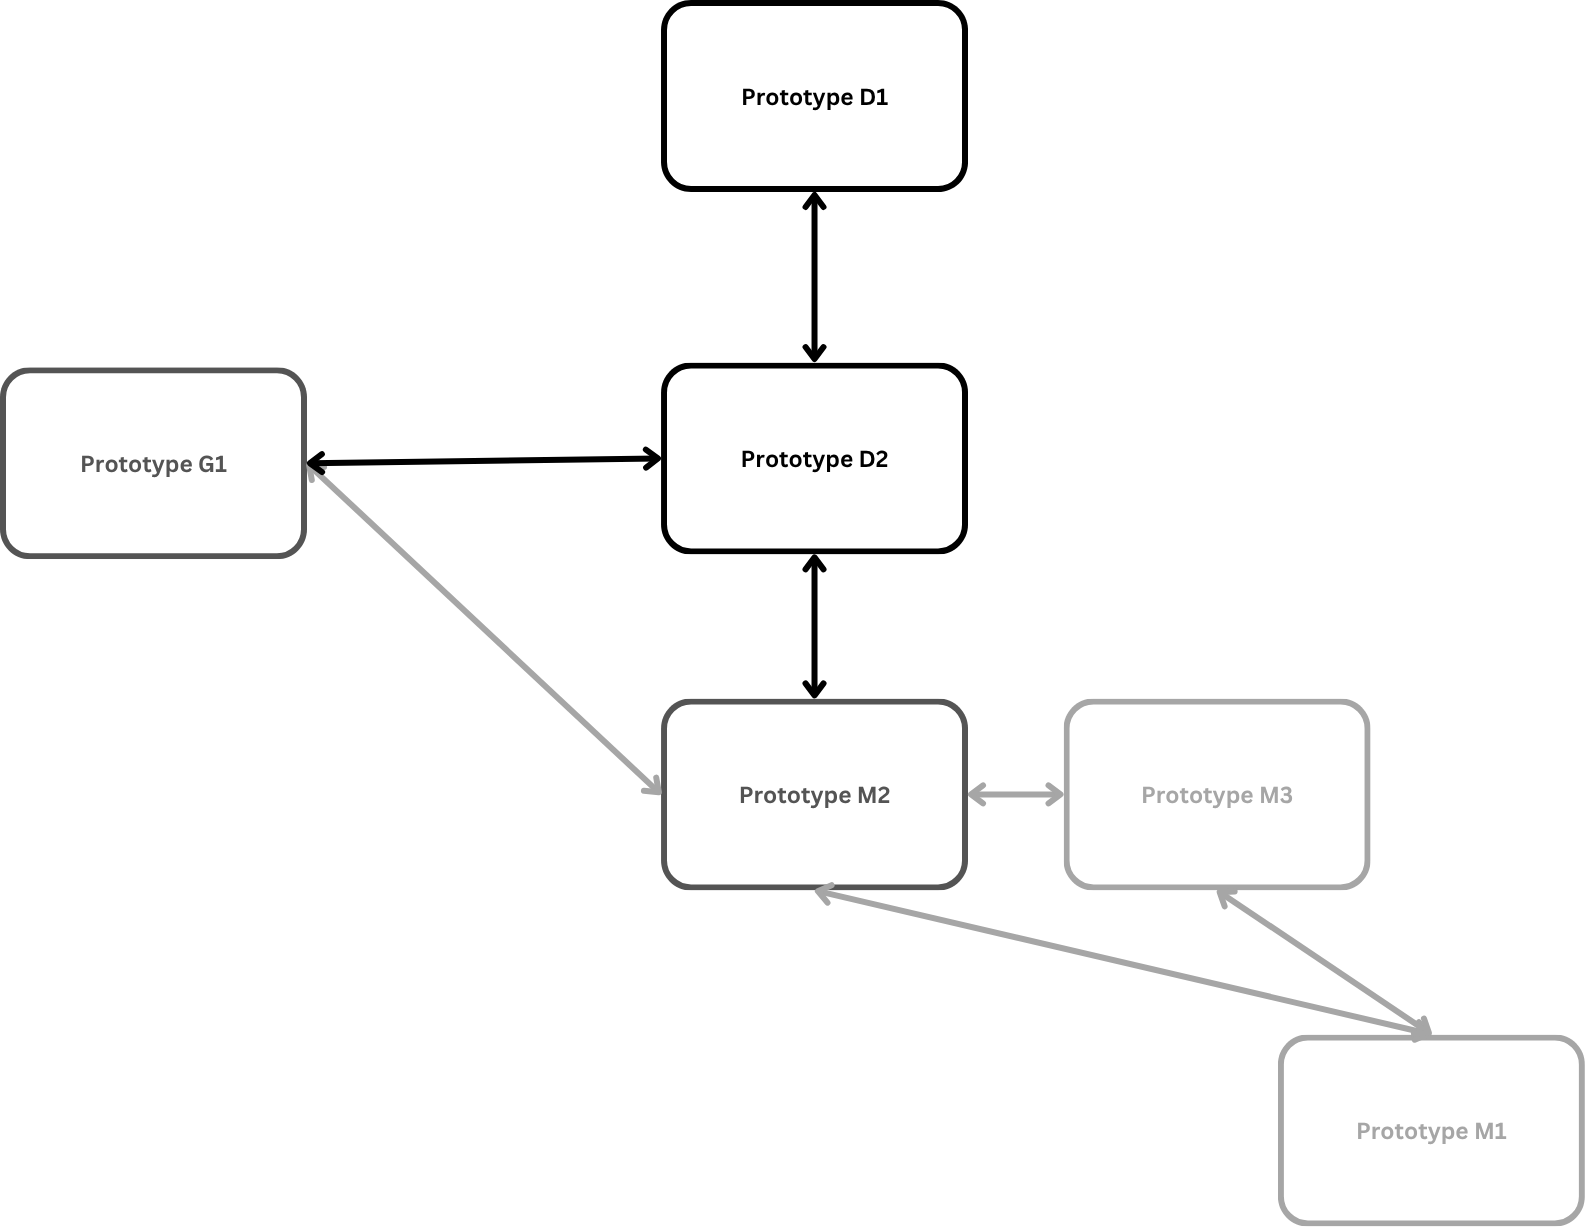
\includegraphics[width=0.7\textwidth]{figs/D-dependencies.png}
    \caption{Dependencies between prototypes of milestone 1 and the rest of the target system, shown by an interaction diagram.}
\end{figure}

\subsection{Architecture analysis}

The requirements describe the need for users to be able to locate files regarding datasets (and models, if it were necessary). Hence, an heterogeneous system will be 
required that is able to load a file or dataset from some sort of initial information, such as an URL. The architecture of this application will be monolithic, but will 
also have the capability to handle connections to remote file systems. Also, the coming prototypes will integrate an automatic version detection system that loads the file and 
sets it in the correct version.

\subsection{Application type analysis}

Since the main objective of this prototype is to locate and load files and perform configuration management operations on them, the most suitable application type is a Wrapper Library 
that covers online and local operations from a machine with authorized access to the file system.

\subsection{Toolkit analysis}

The most suitable toolkits that may serve for the development of this prototype are those related to dataset configuration management (from \emph{Chapter \ref{cap:StateOfTheArt}},
the tool with the most potential was DVC), a toolkit for accessing remote file systems securely and locating files within the local machine, and any toolkit providing a 
mechanism for changing between file versions (the Commit Manager component from prototype \emph{G1} of the system can be used for this purpose).

\subsection{Versioning protocol for datasets}\label{sec:versioningProtocol}

Any dataset integrated within ModelOps will be versioned using the following naming system:

\begin{table}[H]
    \centering
    \begin{tabular}{|c|}
        \hline
        \texttt{<dataset\_name> v<major\_version>.<minor\_version>} \\ \hline
    \end{tabular}
\end{table}

where:

\begin{itemize}
    \item \texttt{<dataset\_name>} is the name of the dataset.
    \item \texttt{<major\_version>} is a positive integer that represents major changes within the datasets without breaking semantics on the purpose of the dataset.
    \item \texttt{<minor\_version>} is a positive integer that represents minor changes within the datasets.
\end{itemize}

\section{PROTOTYPE DESIGN AND DEVELOPMENT}

Within the coming sections, details for the design, implementation and testing phases of the development of this milestone's prototypes are shown in a sequential order. This
milestone is composed of two prototypes, whose development details will be shown in the following subsections.

\subsection{Prototype \emph{D1}}

Prototype D1 consists in the initial stage of development of milestone 1. The objective of this prototype is to 
provide the necessary mechanisms to integrate and transparently locate a dataset within the target system.

\subsubsection{Design for prototype \emph{D1}}

The use case diagram for prototype \emph{D1} is shown in \emph{figure \ref{fig:useCaseD1}}.

\begin{figure}[H]
    \centering
    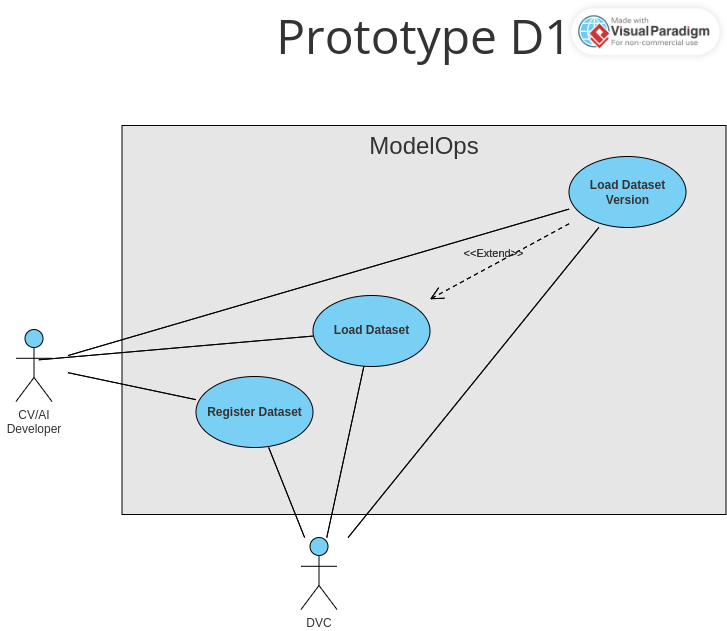
\includegraphics[width=0.7\linewidth]{figs/use-case-D1.png}
    \caption{Use case diagram for prototype \emph{D1}.}
    \label{fig:useCaseD1}
\end{figure}

Two main tasks can be extracted from this use case diagram. The first task is related to the tracking of changes within datasets, focusing particularly on enabling this action on a 
dataset. The second task, additionally, is to enable users to load datasets in either their latest version or any specific existent version. For the fulfillment of 
this objective, two new components will be created, along with a pack of classes to represent exceptions, errors and specific states for a dataset repository.

\paragraph{Prototype \emph{D1} components}

\begin{itemize}
    \item \textbf{Dataset Tracker: }this component will be used for carrying out tasks related with tracking changes on the datasets. For this prototype, it should be 
    capable of starting the change tracking on a dataset and revert its state to a previous, past version.
    
    \item \textbf{Integration States: }an enumeration component that contains the possible states of integration of a dataset repository into ModelOps' configuration management 
    system: Fully integrated, partially or semi integrated or not integrated.
    
    \item \textbf{Dataset Fetchers: }a series of components with the main purpose of providing users with the mechanism to obtain datasets from virtually any location, as well as to 
    load them in their different versions, by means of a unified interface to name the dataset versions. For this prototype, only one implementation of this interface will be made.
    
    \item \textbf{Dataset Exceptions: }a set of exceptions and errors created to represent the possible undesireable or exceptional states that can be encountered by operating 
    the previous two components.

\end{itemize}

\paragraph{Prototype \emph{D1} components' contents}\mbox{}\\

This paragraph will address the question of which information is stored by each of the classes and what functions will be contained within them. The methods of each component 
are described within the following lists.

\subparagraph{Dataset Tracker}\mbox{}\\


The attributes of this component are:

\begin{itemize}
    \item \texttt{dataset\_repo\_path}: a character string that contains the path to a local repository where the dataset is stored. The component 
    will always operate using this repository as reference. This repository may be a DVC repository, a Git repository, both or neither of these.
\end{itemize}

The methods of this component are:

\begin{itemize}
    \item \texttt{integrateDatasetRepo}: start the configuration management lifecycle for a dataset. This enables tracking the changes within any dataset (be it a 
    file or directory) contained within the repository.

    \item \texttt{changeDatasetToVersion}: changes the repository to the selected previous version, reverting the changes made to the tracked items to that version, 
    if they are still tracked by the system on that version. If a list of item paths are passed as parameter, only those will be the ones whose changes will be 
    reverted.

    \item \texttt{isDatasetRepoIntegrated}: support method that checks if the dataset repository has been integrated into MADTrack's configuration management system. 
    It can be used by users and by other classes within the module.

\end{itemize}

\subparagraph{Dataset Fetcher}\mbox{}\\

The only attribute of this interface is:

\begin{itemize}
    \item \texttt{source\_location}: the path to the source repository.
\end{itemize}

The methods of this interface are:

\begin{itemize}
    \item \texttt{fetchDataset}: Method that fetches a dataset from the source location to the target location, then changes its version to the desired one. All of this
    in the same transaction if needed.
\end{itemize}

\subparagraph{Local Dataset Fetcher}\mbox{}\\

This is a especialized class implementing the \emph{Dataset Fetcher} interface, with domain to local repositories. It means this class is able to fetch datasets from a local 
repository to another local repository.

Apart from the attributes and methods inherited from the \emph{Dataset Fetcher} interface, this class has the following methods:

\begin{itemize}
    \item \texttt{createNewDatasetFromLocal}: Method that fetches a dataset from another local repository, then resets the change history to then create a new dataset, 
    which is automatically integrated into MADTrack's configuration management system.
\end{itemize}

\subparagraph{Integration States}\mbox{}\\

The possible states for this enum are:

\begin{enumerate}
    \item \textbf{Not Integrated}.
    \item \textbf{Partially Integrated}.
    \item \textbf{Fully Integrated}.
\end{enumerate}

\paragraph{Prototype \emph{D1} class relationships}\mbox{}\\

Due to the Dataset Fetcher(s) and the Dataset Tracker components being an interface to be implemented by both the local and remote commit managers, they will contain 
an implementation relationship with the Commit Manager component from the \texttt{configuration\_management} module. Now, the relationships among the components are:

\begin{itemize}
    \item Implementation - Local Dataset Fetcher $\rightarrow$ Dataset Fetcher
    \item Dependency - Dataset Fetcher $\rightarrow$ Dataset Exceptions
    \item Dependency - Dataset Tracker $\rightarrow$ Dataset Exceptions
    \item Dependency - Dataset Fetcher $\rightarrow$ Dataset Tracker
    \item Dependency - Dataset Tracker $\rightarrow$ configuration management module (Commit Manager)
    \item Dependency - Dataset Tracker $\rightarrow$ GitPython
    \item Dependency - Dataset Tracker $\rightarrow$ DVC
    \item Dependency - Dataset Tracker $\rightarrow$ Integration States
    \item Dependency - Dataset Fetcher $\rightarrow$ Integration States
\end{itemize}

\paragraph{Prototype \emph{D1} design output}\mbox{}\\

The design for prototype \emph{D1} is shown in \emph{Placeholder for annex figure}.

\subsubsection{Implementation for prototype \emph{D1}}

On the coming paragraphs, details such as the employed programming languages and libraries and other implementation details of prototype \emph{D1} will be shown.

\paragraph{Programming language} \mbox{}\\

Just for the same reasons detailed on the previous chapter, Python is the main programming language of all the possible toolkits and libraries to use. Hence, it will
the choice for the implementation of this prototype.

\paragraph{Libraries} \mbox{}\\

The libraries used for the implementation of this prototype were:

\begin{itemize}
    \item \textbf{\emph{GitPython}: }this toolkit also helped in this prototype, as the Commit Manager has a synergy with the dataset configuration management module.
    \item \textbf{\emph{DVC}: }this library was used to implement the dataset integration and version change functionalities.
    \item \textbf{\emph{Logging}: }A library that enables the creation of log files and manages log operations within any Python application.
    \item \textbf{\emph{OS}: }this library returns for providing repository existence verification mechanisms.
    \item \textbf{\emph{SHutil}: }a library that enables the creation and removal of directories and files. mainly used for developing functionalities for the Local Dataset Fetcher component.
\end{itemize}

\paragraph{Dataset Tracker method flows} \mbox{}\\

\subparagraph{Dataset Tracker - Constructor}

\begin{enumerate}
    \item When the function is called, the code validates the name of the dataset path provided as parameter for security purposes, its existence and its typing as a directory
    (it must be a directory since it is or will be transformed into a Git repository).

    \begin{enumerate}
        \item If some of these validation checks failed, an error would be raised.
    \end{enumerate}

    \item The function stores the aforementioned parameter as an attribute and returns an instance of the class. 
\end{enumerate}

\subparagraph{Dataset Tracker - integrateDatasetRepo}

\begin{enumerate}
    \item When the function is called, the function checks the integration state of the repository.
    \begin{enumerate}
        \item If the integration state of the repository is \emph{Fully Integrated}, the process ends. Making the function idempotent.
        
        \item If the integration state of the repository is \emph{Not Integrated}, Git is initialized in the repository. This operation will be idempotent if the repository is already initialized, so only Git internal errors may happen here.
        Then, the function proceeds to step \emph{c}.

        \item If the integration state of the repository is \emph{Partially Integrated}, the function initializes a DVC repository in the dataset before ending the process.
    \end{enumerate}
\end{enumerate}

\subparagraph{Dataset Tracker - changeDatasetToVersion}

\begin{enumerate}
    \item Upon being called, the function checks the integration state of the repository. Only if it is \emph{Fully Integrated} will the process continue, raising an error otherwise.
    
    \item The function checks the validity of the dataset version name parameter, as well as the version numbers. Any fail in these checks will raise an error.
    
    \item Checkout the repository to the specified version.
    
    \item Recheck the integration state of the repository, since it may not be the same as the one in the initial version. As on step 1, the function will not continue if the repository is not \emph{Fully Integrated}.
    
    \item The action course diverges depending on the presence of a list of strings with the specific dataset items to check out.
    \begin{enumerate}
        \item If no items are entered, the command  checkout will be executed on every item. Any failure will be communicated to the user before ending the process.
        \item If a list of items is provided, the command checkout will be executed for each element of the list after confirming its validity. Any failure will be communicated to the user before continuing the iteration.
    \end{enumerate}
\end{enumerate}

\subparagraph{Dataset Tracker - isDatasetRepoIntegrated}

\begin{enumerate}
    \item Upon being called, it checks the validity of the dataset path and tries to verify it being a Git and a DVC repository.
    \begin{enumerate}
        \item If the dataset is not integrated with Git, the method will return a \emph{Not Integrated} state.
        \item If the dataset is integrated with Git but not with DVC, the method will return a \emph{Partially Integrated} state.
        \item If the dataset is integrated with Git and DVC, the method will return a \emph{Fully Integrated} state.
    \end{enumerate}
\end{enumerate}

\paragraph{Dataset Fetcher method flows} \mbox{}\\

\subparagraph{Local Dataset Fetcher - Constructor}

\begin{enumerate}
    \item When the function is called, the function checks the validity of the source path passed as a trackable dataset using an instance of DatasetTracker.
    \item If the parameter is valid, it is stored as an attribute and the function returns an instance of the class.
\end{enumerate}

\subparagraph{Local Dataset Fetcher - fetchDataset}

\begin{enumerate}
    \item The function checks the validity of the minor and major version parameters. Raising an error if any of them were not valid.
    \item Uses the private function \emph{copyDataset} to copy the dataset to the target location.
    \item If no failures occur, the function ends.
\end{enumerate}

\subparagraph{Local Dataset Fetcher - createNewDatasetFromLocal}

\begin{enumerate}
    \item Upon being called, it uses the function fetchDatasetVersion to copy the dataset to the target location.
    \item The change history is reset to then create a new dataset, which is automatically integrated into MADTrack's configuration management system.
    \item If no failures occur, the function ends.
\end{enumerate}

\subsubsection{Testing for prototype \emph{D1}}

For the testing phase of prototype \emph{D1}, the equivalence classes and test suites will be detailed on this subsection. Additionally, there will be a final section
that will show the errors fixed during this phase.

\paragraph{Equivalence classes for Dataset Tracker} \mbox{}\\

\subparagraph{Dataset Tracker - Constructor} \mbox{}\\
\begin{enumerate}
    \item The path to the dataset does not pass the string validation check.
    \item The path to the dataset passes the string validation check, but does not exist.
    \item All of the above is passed, but now the dataset is no directory.
    \item Every parameter and validation check goes fine.
\end{enumerate}

\subparagraph{Dataset Tracker - integrateDatasetRepo} \mbox{}\\
\begin{enumerate}
    \item The dataset is not integrated.
    \item The dataset repository is already integrated.
\end{enumerate}

\subparagraph{Dataset Tracker - changeDatasetToVersion} \mbox{}\\
\begin{enumerate}
    \item The dataset repository is not integrated.
    \item The dataset name does not pass the string validation check.
    \item Either version number parameter does not pass the validation check.
    \item The specified dataset does not exist.
    \item Before checking out, the list of passed parameters is an empty list.
    \item All parameters are valid.
\end{enumerate}

\subparagraph{Dataset Tracker - isDatasetRepoIntegrated} \mbox{}\\
\begin{enumerate}
    \item The dataset is not a Git repository.
    \item The dataset is a Git repository, but not a DVC repository.
    \item The dataset is a Git repository and a DVC repository.
\end{enumerate}

\subparagraph{Dataset Fetcher - Constructor} \mbox{}\\
\begin{enumerate}
    \item The source location parameter is not valid.
    \item The source location parameter is a valid, tracked dataset.
\end{enumerate}

\subparagraph{Dataset Fetcher - fetchDataset} \mbox{}\\
\begin{enumerate}
    \item The target location is not valid.
    \item The major version parameter is not valid.
\end{enumerate}

\subparagraph{Dataset Fetcher - createNewDatasetFromLocal} \mbox{}\\
\begin{enumerate}
    \item The dataset location is not valid.
    \item The version parameters are not valid
    \item Every parameter is valid.
\end{enumerate}

\paragraph{Test suites for prototype \emph{D1}}\mbox{}\\

The test suites for this class can be found in \emph{annex reference placeholder}. % Referencia al Anexo con las tablas (porque pueden ser muy grandes y no es plan). Esto no es prioritario, puede esperar

\paragraph{Errors found and lessons learned during the development of prototype \emph{D1}}\mbox{}\\

The errors encountered during the course of the testing phase of prototype \emph{G1} are shown in \emph{annex reference placeholder}. % De nuevo, esto puede esperar porque va al anexo

\subsection{Prototype \emph{D2}}

Prototype D2 is the second stage of development of Milestone 1. The objective of this prototype is to provide the necessary mechanisms to commit changes to a dataset.

\subsubsection{Design for prototype \emph{D2}}

The output of the design for prototype \emph{D2} is developed by designating the various components that make up this prototype, their contents and their connection with the rest of the system.
Hence, the design details for this prototype are shown in the following paragraphs.

\paragraph{Components for prototype \emph{D2}} \mbox{}\\

The use case diagram is shown in \emph{figure \ref{fig:useCaseD2}}.

\begin{figure}[H]
    \centering
    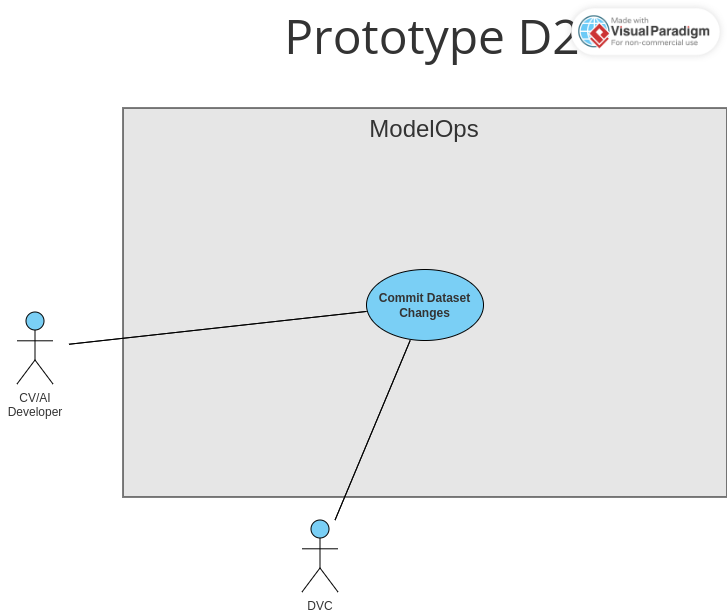
\includegraphics[width=0.7\linewidth]{figs/use-case-D2.png}
    \caption{Use case diagram for prototype \emph{D2}.}
    \label{fig:useCaseD2}
\end{figure}

The main task is to perform commits over a dataset. For this objective, the Dataset Tracker component can be used, as it already has a function that allows the user to 
commit changes to a dataset and generate a new version of it. Hence, the involved components are:

\begin{itemize}
    \item \textbf{Dataset Tracker: }this class will be used for carrying out tasks related with tracking changes on the datasets. For this prototype, it should be capable of creating new versions of a dataset and upload them to a local or remote repository.
\end{itemize}

\paragraph{Components' contents for prototype \emph{D2}} \mbox{}\\

All of the contents added in this prototype belong to the Dataset Tracker component.

\paragraph{Dataset Tracker} \mbox{}\\

This component gained a new method for this prototype:

\begin{itemize}
    \item \texttt{trackDatasetChanges: }given a directory or file path within the integrated dataset repository, commits its changes using MADTrack's dataset 
    configuration management system. This means that if this is the first commit made to the item using MADTrack, the necessary mechanisms will be added to the 
    repository to first register it as a tracked dataset.
\end{itemize}

\paragraph{Class relationships for prototype \emph{D2}} \mbox{}\\

The dependencies among classes do not change in comparison with the previous prototype. Hence, the relationships will be kept the same.

\paragraph{Design output for prototype \emph{D2}}\mbox{}\\

The design class diagram for prototype D2 is shown in \emph{Placeholder for annex figure}.

\subsubsection{Implementation for prototype \emph{D2}}

Prototype \emph{D2} mostly follows the same implementation details as the previous prototype of the milestone. Following Python as the main programming language and the same
libraries. Therefore, the only thing remaining is to detail the flow of the new method.

\paragraph{Dataset Tracker method flows} \mbox{}\\

\subparagraph{Dataset Tracker - trackDatasetChanges} \mbox{}\\

\begin{enumerate}
    \item When the function is called, the function checks the integration state of the repository. Only if it is \emph{Fully Integrated} will the process continue.
    \item The function checks the validity of the dataset path and dataset version name, as well as the existence of the dataset within the repository.
    \item The function checks the validity of the dataset version numbers. They must not be negative.
    \item The name of the dataset version is built automatically following the established order (see \emph{section \ref{sec:versioningProtocol}}), and the system checks whether the version already exists in the repository, raising an error if that is the case.
    \item Given the dataset version is valid, dvc is called to track the dataset in the repository.
    \begin{enumerate}
        \item In case this dataset is already tracked by DVC, it will update the change index file to generate a new version of it.
    \end{enumerate}

    \item Finally, the function commits the changes made to the repository using the version name as the commit message.
    \begin{enumerate}
        \item If the remote flag is set, the function will execute a remote commit process.
    \end{enumerate}
\end{enumerate}

\subsubsection{Testing for prototype \emph{D2}}

The testing phase of prototype \emph{D2} was clearly focused on testing the new method. Its test suites can be found at \emph{annex reference placeholder} and the errors fixed can be found at \emph{annex reference placeholder}.
With reference to the equivalence classes, they can be found below.

\paragraph{Equivalence classes for Dataset Tracker} \mbox{}\\

\subparagraph{Dataset Tracker - trackDatasetChanges} \mbox{}\\

\begin{enumerate}
    \item The dataset is not integrated.
    \item The dataset item path is an invalid string.
    \item The dataset version name is an invalid string.
    \item Any of the version number parameters are invalid.
    \item The specified dataset does not exist within the repository.
    \item The specified dataset repo version is already registered.
    \item All the parameters are valid.
\end{enumerate}

